\section{Gestione di configurazione}\label{s:configurazione}

Per la configurazione del prodotto e per la gestione documentale vengono utilizzate varie strategie per organizzare e rendere consistente.

\subsection{VCS}\label{sss:vcs} Per il versionamento e tracciamento delle modifiche apportate ai documenti e al codice steso durante il progetto viene utilizzato il \textit{version control system} Git. 

In abbinata a Git viene utilizzato GitHub per permettere facile collaborazione oltre ad accorpare in un unico luogo anche gli strumenti di ITS e CI/CD pipeline.

\subsection{ITS} Per il tracciamento delle issue viene utilizzato GitHub.

\subsubsection{Etichette} 

    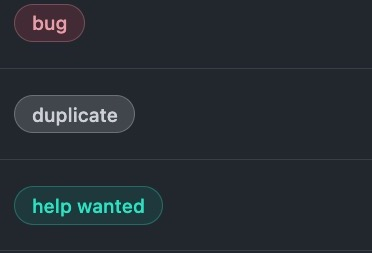
\includegraphics[width=0.49\linewidth]{img/etichette.jpeg}
    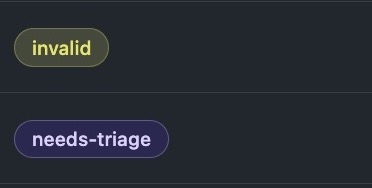
\includegraphics[width=0.49\linewidth]{img/etichette2.jpeg}

Per migliorare la visione e l'organizzazione delle issue vengono usate delle etichette standard per ogni repository, oltre a etichette specifiche analizzate repository per repository.

\begin{table}[h]
    \centering
    \begin{tabularx}{\linewidth}{l | X}
        \textbf{Etichetta} & \textbf{Scopo}\\
        \hline
        \textbf{bug} & Segnala che la issue è relativa ad un bug \\
        \textbf{duplicate} & Poichè le issue possono essere aperte da ognuno del gruppo è possibile che ci si creino due issue simili, questa etichetta denota la seconda delle due come duplicata \\
        \textbf{help wanted } & Etichetta di default di \textit{GitHub} che denota issue da gestire in più persone o che si sono fermate per via di imprevisti\\
        \textbf{invalid} & Se quanto scritto nella issue non è attinente oppure è diventato obsoleto prima del completamento, questa issue ne denota l'invalidità\\
        \textbf{needs-triage} & Quando una issue viene aperta per la prima volta non da un responsabile, ottiene questa etichetta \\
    \end{tabularx}
    \caption{Tipologie di etichette}
    \label{table:t_etichette}
\end{table}

\subsubsection{Ciclo di vita di una issue}\label{sss:triage}

\paragraph{Nota per il lettore} Si consiglia la visione della parola \textit{triage} nel glossario.

Quando viene deciso o proposto un cambiamento, quando si affermano problemi tecnici o quando ci sono questioni da affrontare, viene aperta una issue.

Una issue\footnote{Si consiglia la visione della sezione \ref{sss:issue}} deve contenere tutte le informazioni affinché la questione posta possa essere affrontata e risolta.

I cicli di vita delle issue sono i seguenti:

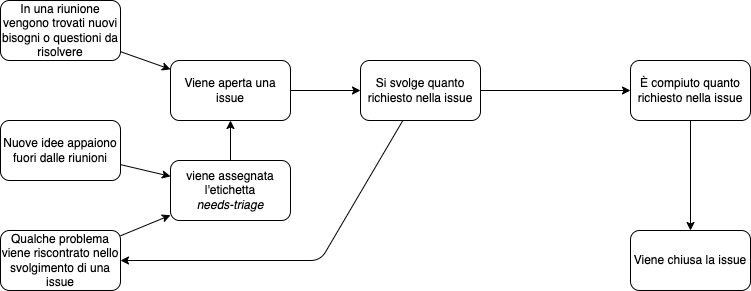
\includegraphics[width=\linewidth]{img/ciclo-vita-issue.png}

\subsubsection{Apertura di una issue}\label{sss:issue}

Una issue deve raccontare nel modo più semplice e veloce possibile una problematica oppure un bisogno.

Una issue deve contenere al suo interno la motivazione dell'apertura e il requisito che ne può determinare la chiusura.

Una issue deve essere pensata come una questione risolvibile da una persona sola, se così non è\footnote{A meno di casi estremi.} la issue va segmentata in issue più piccole e gestibili da singoli in un tempo minore o uguale alla lunghezza di uno sprint.


\subsection{Strutturazione dei repository}

Nel sistema di controllo del versionamento sono presenti due tipologie di repository:

\begin{itemize}
    \item \textbf{Repository documentale}: dedicato al sorgente in tex dei documenti;
    \item \textbf{Repository codice-sorgente}: dedicato al sorgente dei vari software.
\end{itemize}

\paragraph{Documentazione} Per la documentazione si è scelto un approccio a sottomoduli. Per ognuno dei documenti viene definito un singolo repository. Per la consegna degli artefatti rilasciati al \textit{Committente} e al \textit{Proponente} viene però utilizzato un repository centrale unico, contenente tutti i sottomoduli documentali.

\begin{center}

\includegraphics[width=0.6\linewidth]{img/struttura-repo-doc.png}
\end{center}
